\documentclass{standalone}

\usepackage[english]{babel}
\usepackage[linesnumbered, ruled, vlined]{algorithm2e}

\usepackage{caption}

% to create listings

\usepackage{listings, lstautogobble}
\lstset{
  autogobble=true,
  frame=single,
}

\lstdefinelanguage{coq}[Objective]{Caml}{
  morekeywords={Structure, Definition, Inductive, list, return},
  sensitive=true
}

% to define font size

\usepackage{ulem}
\usepackage{moresize}
\usepackage{anyfontsize}

% to use tikz and its libraries

\usepackage{tikz-timing}
\usepackage{tikz}

\usetikzlibrary{backgrounds}
\usetikzlibrary{positioning, calc, arrows, shapes, automata, petri, patterns}

% to use tikzmark, to place and refer to marks outside the current figure

\tikzset{every picture/.style={remember picture}}

% styles for transitions

\tikzset{transition/.append style={fill=black!20, thick}}
\tikzset{transition/.append style={fill=black!20, thick}}

% styles for test and inhib arcs.

\tikzstyle{test}=[pre, *-]
\tikzstyle{inhib}=[pre, o-]

% to use colors

\usepackage{xcolor}
\usepackage{MnSymbol}

%%%%%%%%%%%%%%%%%%%%%%%%%%%%%%%%%%%%%%%%%%%%%%%%%%
%                  BEGIN DOCUMENT                %
%%%%%%%%%%%%%%%%%%%%%%%%%%%%%%%%%%%%%%%%%%%%%%%%%%

\newcommand{\on}[2]{\mathop{#1}\limits_{}^{#2}}

\begin{document}

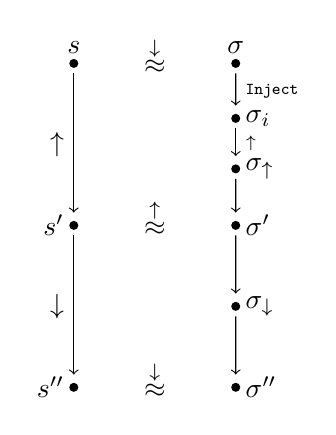
\begin{tikzpicture}

  % POINTS
  
  \node (spoint) [draw,circle,fill=black,inner sep=1pt]{};
  \node (sppoint) [draw,circle,fill=black,inner sep=1pt] at ($(spoint.south)-(0,2)$) {};
  \node (sspoint) [draw,circle,fill=black,inner sep=1pt] at ($(sppoint.south)-(0,2)$) {};
  
  \node (sigpoint) [draw,circle,fill=black,inner sep=1pt] at ($(spoint.east)+(2,0)$) {};
  \node (sigppoint) [draw,circle,fill=black,inner sep=1pt] at ($(sppoint.east)+(2,0)$) {};
  \node (sigspoint) [draw,circle,fill=black,inner sep=1pt] at ($(sspoint.east)+(2,0)$) {};

  \node (sigrepoint) [draw,circle,fill=black,inner sep=1pt] at ($(sigpoint.south)!.66!(sigppoint.north)$) {};
  \node (sigfepoint) [draw,circle,fill=black,inner sep=1pt] at ($(sigppoint.south)!.5!(sigspoint.north)$) {};

  \node (siginjrpoint) [draw,circle,fill=black,inner sep=1pt] at ($(sigpoint.south)!.33!(sigppoint.north)$) {};
  % \node (siginjfpoint) [draw,circle,fill=black,inner sep=1pt] at ($(sigppoint.south)!.33!(sigspoint.north)$) {};
  
  \node at ($(spoint)!0.5!(sigpoint)+(0,3pt)$) {$\stackrel{\downarrow}{\approx}$};
  \node at ($(sppoint)!0.5!(sigppoint)+(0,3pt)$) {$\stackrel{\uparrow}{\approx}$};
  \node at ($(sspoint)!0.5!(sigspoint)+(0,3pt)$) {$\stackrel{\downarrow}{\approx}$};

  % % LABELS

  % % POINT LABELS.

  \node[anchor=south] (slabel) at ($(spoint)$) {$s$};
  \node[anchor=east] (splabel) at ($(sppoint)$) {$s'$};
  \node[anchor=east] (sslabel) at ($(sspoint)$) {$s''$};
  
  \node[anchor=south] (siglabel) at ($(sigpoint)$) {$\sigma$};
  \node[anchor=west] (sigrelabel) at ($(sigrepoint)$) {$\sigma_\uparrow$};
  \node[anchor=west] (sigplabel) at ($(sigppoint)$) {$\sigma'$};
  \node[anchor=west] (sigfelabel) at ($(sigfepoint)$) {$\sigma_\downarrow$};
  \node[anchor=west] (sigslabel) at ($(sigspoint)$) {$\sigma''$};
  \node[anchor=west] (siginjrlabel) at ($(siginjrpoint)$) {$\sigma_{i}$};
  % \node[anchor=west] (siginjflabel) at ($(siginjfpoint)$) {$\sigma'_{i}$};
  

  % SQUIGGY PATH LABELS.
  
  \node[anchor=east] at ($(spoint)!0.5!(sppoint)$) {$\uparrow$};
  \node[anchor=east] at ($(sppoint)!0.5!(sspoint)$) {$\downarrow$};

  \node[anchor=west] at ($(sigpoint)!0.5!(siginjrpoint)$) {\fontsize{6}{8}\selectfont $\mathtt{Inject}$};
  \node[anchor=west] at ($(siginjrpoint)!0.5!(sigrepoint)$) {\fontsize{6}{8}\selectfont $\uparrow$};
  \node[anchor=west] at ($(sigrepoint)!0.5!(sigppoint)$) {\fontsize{6}{8}\selectfont $\downlsquigarrow$};
  % \node[anchor=west] at ($(sigppoint)!0.5!(siginjfpoint)$) {\fontsize{6}{8}\selectfont $\mathtt{Inject_\downarrow}$};
  % \node[anchor=west] at ($(siginjfpoint)!0.5!(sigfepoint)$) {\fontsize{6}{8}\selectfont $\downarrow$};
  \node[anchor=west] at ($(sigfepoint)!0.5!(sigspoint)$) {\fontsize{6}{8}\selectfont $\downlsquigarrow$};
  
  
  % SQUIGGY PATHS

  % SITPN state squiggy paths
  
  \path[draw,->] 
  ($(spoint.south)-(0,2pt)$) -- ($(sppoint.north)+(0,3pt)$);

  \path[draw,->]
  ($(sppoint.south)-(0,2pt)$) -- ($(sspoint.north)+(0,3pt)$);

  % VHDL design state squiggy paths

  \path[draw,->]
  ($(sigpoint.south)-(0,2pt)$) -- ($(siginjrpoint.north)+(0,3pt)$);

  \path[draw,->]
  ($(siginjrpoint.south)-(0,2pt)$) -- ($(sigrepoint.north)+(0,3pt)$);

  \path[draw,->]
  ($(sigrepoint.south)-(0,2pt)$) -- ($(sigppoint.north)+(0,3pt)$);

  \path[draw,->]
  ($(sigppoint.south)-(0,2pt)$) -- ($(sigfepoint.north)+(0,3pt)$);

  \path[draw,->]
  ($(sigfepoint.south)-(0,2pt)$) -- ($(sigspoint.north)+(0,3pt)$);
  
\end{tikzpicture}

\end{document}
%%% Local Variables:
%%% mode: latex
%%% TeX-master: t
%%% End:
